\subsection{Leakage from augmented copies}
Table~\ref{tab:leak} and Fig.~\ref{fig:leak} compare the per-file and grouped
protocols. Under the per-file split every EfficientNet-B0 seed classifies every
test image correctly (\NaiveFreshAcc\% freshness, \NaiveTypeAcc\% type). The
grouped split lowers this to \MtlFreshAcc\% and \MtlTypeAcc\%. The effect is
larger for the colour-histogram baseline, whose freshness accuracy drops from
\HistNaiveFreshAcc\% to \HistGroupedFreshAcc\% and type accuracy from
\HistNaiveTypeAcc\% to \HistGroupedTypeAcc\%: the per-file split lets even a
model with no spatial features look almost as good as a deep network, which
hides how much of the task the CNN actually solves.

\begin{figure}[t]
\centering
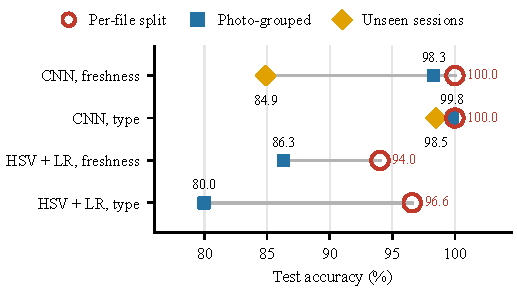
\includegraphics[width=\columnwidth]{figures/leakage.pdf}
\caption{Test accuracy under the per-file and grouped splits.}
\label{fig:leak}
\end{figure}

\subsection{Session-level dependence}
Grouping by source photo does not make test images independent of training.
File names indicate only \NSessions{} capture sessions (a capture date or
camera series within a class; we infer them from file-name patterns), and \SessionSharePct\% of grouped-split test images
come from a session that also contributes training images; \NSingleSessionStrata{}
of the 12 produce/freshness strata consist of a single session. For the
\NHeldOutStrata{} strata with more than one session we built a held-out-session
split (\NSessTrain{}/\NSessVal{}/\NSessTest{} images) in which each such stratum
contributes one entire, unseen session to the test set. We drop the
\NSessExcluded{} training images that are augmented copies (same file-name
source) or near-duplicates (dHash within 2 bits) of a test image; no remaining
training image is within 2 bits of a test image. Clusters from the grouped
split may still span train and test here, because chained merging links
different photographs of the same session, which is exactly the dependence
this protocol probes.

On this split freshness accuracy is \SessFreshAcc\% (vs.\ \MtlFreshAcc\% on the
grouped split), while produce-type accuracy stays at \SessTypeAcc\%, and the
freshness ECE rises from \MtlFreshEce\% to \SessFreshEce\%: the model becomes
confidently wrong. Table~\ref{tab:session} breaks this down by stratum. On the
\NSessCommonStrata{} strata that also occur in the grouped test, accuracy falls
only from \SessStrataGroupedFreshAcc\% to \SessStrataHeldFreshAcc\%; apple,
bitter gourd and orange sessions transfer almost perfectly. The failures are
capsicum (\SessHeldCapsicumFresh\% on an unseen fresh session,
\SessHeldCapsicumStale\% on an unseen stale session) and fresh tomato
(\SessHeldTomatoFresh\%). In both cases the held-out session's capture source
appears in training only with the opposite label: every stale capsicum left in
training is a WhatsApp-compressed photograph, while every camera (IMG-series)
capsicum in training is fresh, so camera photographs of stale capsicums are
called fresh; likewise, all IMG-series tomatoes in training are stale, and the
held-out IMG-series fresh tomatoes are often called stale. This pattern is consistent with
the network having partly learned the acquisition source, a shortcut that
per-file and per-photo splits cannot reveal because \SessionSharePct\% of their
test images share a capture session with training images.

\subsection{Multi-task versus single-task learning and backbones}
Table~\ref{tab:main} reports the grouped-split results. The multi-task
EfficientNet-B0 reaches \MtlFreshAcc\% freshness and \MtlTypeAcc\% type
accuracy, against \FreshFreshAcc\% and \TypeTypeAcc\% for the single-task
networks. The differences are below one percentage point and point in
opposite directions (freshness favours the multi-task model, type the
single-task one); three seeds cannot resolve them, so we find no evidence that
joint training helps or hurts, while one shared network halves inference cost. MobileNetV3-Large matches
EfficientNet-B0 (\MnvFreshAcc\% and \MnvTypeAcc\%) with \MnvParams{}\,M
parameters and \MnvCpuMs{}\,ms CPU latency against \MtlCpuMs{}\,ms, and is the
model we deploy. For a single seed-0 run the 95\% group-bootstrap interval of
freshness accuracy is \MtlSzeroFreshCI{}\%, reflecting that the \NTestGroups{}
test groups, not the \NTest{} images, are the independent units.

\subsection{Cross-dataset produce type}
On \NCross{} external images of five of the six produce types (bell pepper is
mapped to capsicum; there is no bitter gourd), type accuracy is only
\MnvCrossTypeAcc\% (MobileNetV3) and \MtlCrossTypeAcc\% (EfficientNet-B0),
compared with about 99\% in-domain. The external set has no freshness labels;
MobileNetV3 calls \MnvCrossShareFreshExact\% of these retail-style photos fresh
and EfficientNet-B0 \MtlCrossShareFreshExact\%, which is plausible but not an
accuracy.

\subsection{Out-of-distribution gate}
Table~\ref{tab:ood} compares post-hoc scores. Scores computed on the six-way
produce-type head separate in- from out-of-distribution images much better
than scores on the binary freshness head (near-OOD AUROC
\MnvEnergyNearAuroc\% for energy on the type head vs.\ \MnvMspFreshNearAuroc\%
for MSP on the freshness head). For a two-class head, entropy is a monotone
function of MSP, so entropy ranks inputs exactly like MSP. The previous
version of the system rejected an input when freshness entropy exceeded
1.5 bits or its maximum probability fell below 0.3; for a two-class head
neither condition can occur (entropy is at most 1 bit and the maximum
probability at least 0.5), so that gate never fired. With the threshold set at
95\% validation TPR, the MobileNetV3 energy gate, averaged over three seeds,
accepts \MnvGateTestIdAcceptRate\% of in-distribution test images and rejects
\MnvGateFarOODRejectRate\% of CIFAR-10 images but only
\MnvGateNearOODRejectRate\% of unseen produce (\MnvGateNearMin--\MnvGateNearMax\%
across seeds; the deployed seed: \DeployGateAccept\%, \DeployGateFar\% and
\DeployGateNear\%). A photo of an unsupported vegetable is the hard case.
